\chapter[Fundamentação Teórica]{Fundamentação Teórica}
\label{cp:fundamentacao}

\section{Gerenciamento de Projetos}

\subsection{Modelo Tradicional}

Uma metodologia de gerenciamento de projetos no modelo tradicional, de acordo com \cite{kerzner} é o alcance da excelência no gerenciamento de projetos se torna impossível sem um processo repetitivo que possa ser utilizado em cada projeto.

No modelo tradicional, um dos mais modelos mais utilizados é o RUP \textit{(Rational Unified Process)}. O RUP oferece uma metodologia responsável por responder questões como boas práticas para o gerenciamento de projetos, com o objetivo de estruturar e formatar os processos associados às atividades que envolvem a tecnologia de informação. 

As 4 fases principais do RUP podem ser vistas na figura \ref{img:fases_do_rup}:

\begin{figure}[H]
	\centering
	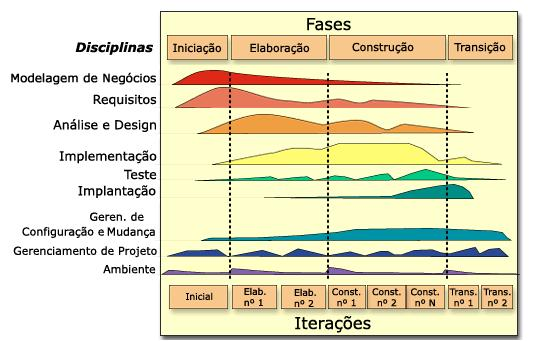
\includegraphics[width=0.8\textwidth]{figuras/fases_rup.jpg}
	\caption{Fases do RUP. Fonte: \cite{rup}.}
	\label{img:fases_do_rup}
\end{figure}

O desenvolvimento do plano de gerenciamento do projeto é uma atividade iterativa ao longo do ciclo de vida do projeto, sempre pronto para melhoria contínua e permitindo à equipes do projeto definir e trabalhar com maior nível de detalhes. De acordo com o \cite{pmbok}, as fases do \cite{rup} são sobrepostas, ou seja, o início de uma fase é ao término de uma outra, isso leva a algumas atividades ocorrerem de forma paralela. A maneira como este tipo de projeto aumenta os riscos, retrabalhos, e exigir recursos adicionais para permitir as atividades em paralelo, como mostrado na figura \ref{img:fases_do_rup}.

Nesta perspectiva, se tem o papel do gerente de projeto como um líder responsável por liderar a equipe para alcançar os objetivos previstos no planejamento do projeto. Entre as funções destes líderes se tem:

\begin{itemize}
    \item Conhecimento acerca do gerenciamento de projetos;
    \item Desempenho para aplicar seus conhecimentos na prática;
    \item Comportamento pessoal de liderança, atingindo objetivos e equilibrando restrições.
\end{itemize}

Este tipo de gerenciamento de projeto é mais utilizado em empresas já consolidadas, de ramo mais formal, que possui mais burocracia em seus projetos e por tanto maior rigor de documentação e de liderança dos gerentes de projeto. Essa hierarquia pode ser vista na figura \ref{img:gerencia_de_projetos_tradicional}.

\begin{figure}[H]
	\centering
	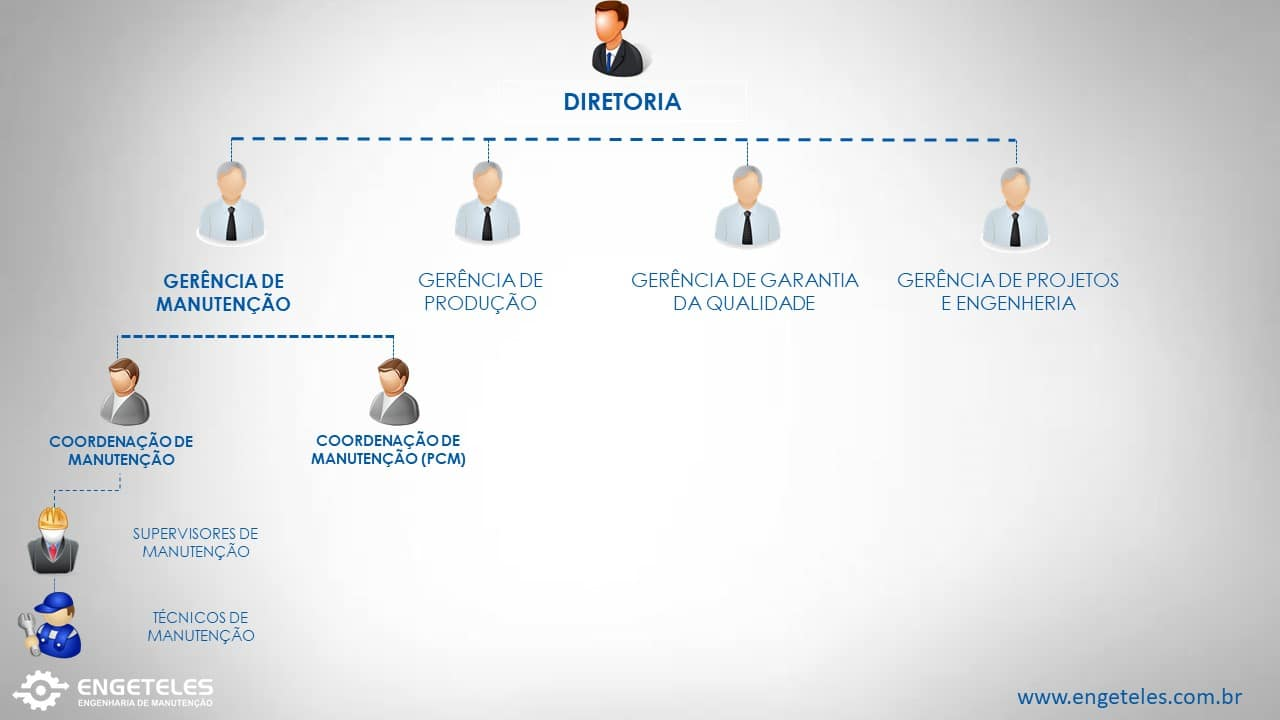
\includegraphics[width=0.8\textwidth]{figuras/gerencia_de_projeto.jpg}
	\caption{Hierarquia em projetos tradicionais. Fonte: \cite{gerentes_tradicionais}.}
	\label{img:gerencia_de_projetos_tradicional}
\end{figure}

\subsection{Modelo Ágil}

Em contraposição ao modelo tradicional, surte o manifesto ágil como uma reação contra o processo burocrático presente no modelo tradicional, que possuem por característica atividades sequências em modelo cascata. Segundo a \cite{chaos} apenas 16,2\% dos projetos entregues por companhias americanas foram entregues respeitando prazos, custos previamente acordados e objetivos determinados. Segundo a própria \cite{chaos}, as principais causas destes problemas estavam relacionadas com o modelo sequencial tradicional.

O modelo ágil, segundo \cite{soares}, ela deve primeiro aceitar as mudanças em vez de tentar prevê-las, agir de maneira rápida sabendo receber, avaliar e responder como elas devem ser respondidas. As principais características da metodologia ágil são:

\begin{itemize}
	\item Desenvolvimento iterativo e incremental;
	\item Comunicação;
	\item Documentação extensiva; 
\end{itemize}

Em 2001, membros da comunidade de \textit{software} se reuniram e criaram o \cite{agile_manifest}. O objetivo deste manifesto é utilizar as melhores práticas observadas em projetos anteriores que obtiveram sucessos.

Os principais conceitos do manifesto ágil são:

\begin{itemize}
	\item Indivíduos e interações ao invés de processos e ferramentas;
	\item \textit{Software} executável ao invés de documentação;
	\item Colaboração do cliente ao invés de negociação de contratos;
	\item Resposta rápida a mudanças ao invés de seguir planos pré-estabelecidos.
\end{itemize}

Uma das boas práticas adotadas ao modelo ágil é o SCRUM. O SCRUM, se refere ao jogo \textit{Rugby}, que é a ação dos jogadores se organizarem em círculo para planejar a próxima jogada. Um dos principais pontos de vista do SCRUM é mostrar um projeto com pequenos ciclos, aumentando as iterações entre os participantes, mas com visão a longo prazo.

O ciclo de vida pode ser visto na figura \ref{img:ciclo_de_vida_scrum}:

\begin{figure}[H]
	\centering
	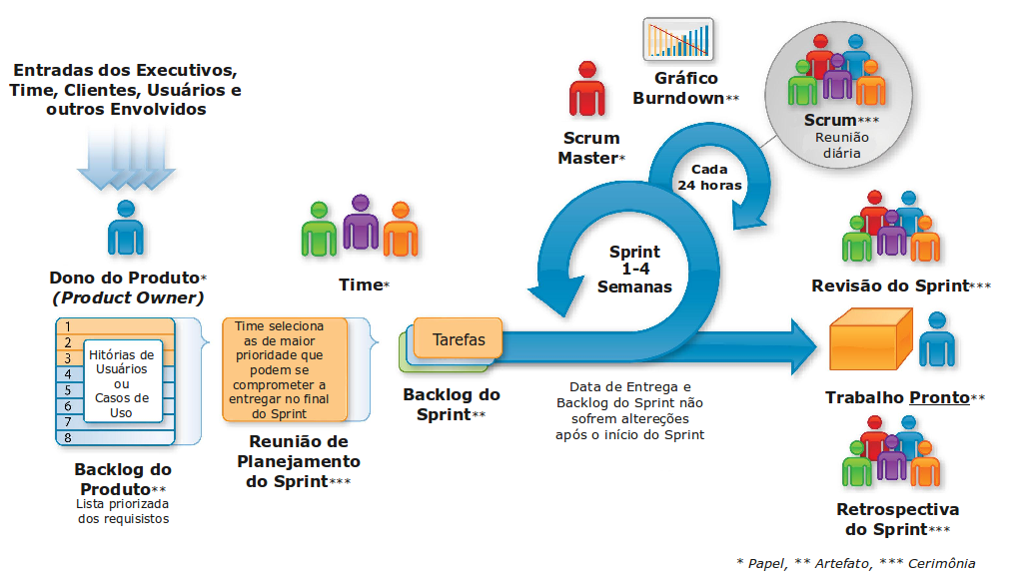
\includegraphics[width=0.8\textwidth]{figuras/ciclo_de_vida_scrum.png}
	\caption{Ciclo de Vida SCRUM. Fonte: \cite{scrum}.}
	\label{img:ciclo_de_vida_scrum}
\end{figure}

Como visto na figura \ref{img:ciclo_de_vida_scrum}, o SCRUM é um ciclo progressivo de várias iterações bem definidas, denominadas \textit{Sprints}. As \textit{Sprints} podem ter duração de uma a quatro semanas. Antes de cada \textit{Sprint}, deve ser realizada a reunião de planejamento da \textit{Sprint}, chamada de \textit{Sprint Planning Meeting}, na qual os desenvolvedores tem contato com o \textit{Product Owner}, que possui o dever de priorizar as atividades, seleciona-las e estimar as tarefas que a equipe pode desenvolver na próxima \textit{Sprint}.

Com o objetivo de saber o progresso de cada equipe dentro da \textit{Sprint}, ocorrem as reuniões diárias, denominadas \textit{Daily Meetings}, que tem duração de no máximo 15 minutos e ocorrem com todos os participantes em pé, respondendo perguntas como: "O que você fez ontem?", "O que você fez hoje?" e "O que você vai fazer amanhã?". 

Ao final de uma \textit{Sprint} é feita uma análise gráfico do progresso do projeto atráves do \textit{Sprint Backlog} durante a \textit{Sprint Review}. Após a \textit{Sprint Review} ocorre a \textit{Sprint Restrospective} que é a análise de experiências que ocorreram durante a \textit{Sprint} sejam boas ou não a fim de melhora-las.

Segundo \cite{fowler}, as equipes devem possuir um quadro para registro das atividades, denominado \textit{Kanban}. O \textit{Kanban} possui o objetivo de auxiliar as equipes em relação ao progresso da \textit{Sprint}, esse quadro pode ser dividido em 4 fases:

\begin{itemize}
	\item Para fazer;
	\item Em andamento (com o nome do responsável pela atividade);
	\item Em revisão;
	\item Feito.
\end{itemize}

\begin{figure}[H]
	\centering
	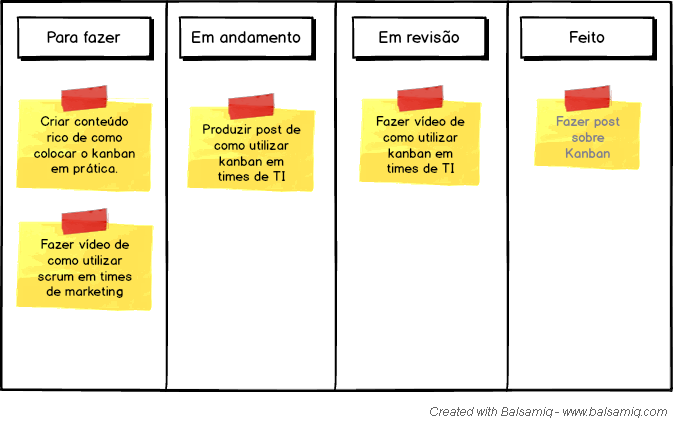
\includegraphics[width=1.0\textwidth]{figuras/kanban.png}
	\caption{Quadro Kanban. Fonte: \cite{kanban}.}
	\label{img:kanban}
\end{figure}

No modelo ágil os requisitos dos clientes podem ser mudados a qualquer momento, e o time de gerência e desenvolvimento devem estar preparados para conversar com o cliente a fim de resolver as alterações de requisitos da melhor maneira possível. Este tipo de pensamento no modelo tradicional é mais difícil de acontecer, pois ao observar a figura \ref{img:fases_do_rup}, é possível notar ao iniciar uma fase, essa mesma fase não é retornada mais tarde, ou seja, no modelo tradicional uma troca de requisitos pode levar ao reinicio do projeto.

Este modelo é mais focado para empresas emergentes, que não são muito rigorosas em seus processos e aceita que mudanças nos requisitos ou na visão do produto são sempre bem vindas, desde que melhore o projeto final.

\section{Desempenho de Reuniões}

\subsection{Modelo Tradicional}

\subsection{Modelo Ágil}

\section{A Instituição}

Tendo a justificativa para o projeto no tópico \ref{sec:justificativa}, seguida do problema de pesquisa (\ref{sec:problema_de_pesquisa}) e os objetivos descritos no tópico \ref{sec:objetivos}, se tem a necessidade de escolher alguma empresa que será usada como caso de estudo para o projeto, no caso foi definido o NMIL (Núcleo de Modernização da Informação Legislativa), um setor localizado no Senado Federal Brasileiro.

\subsection{Senado Federal}

As funções do Senado Federal são exercidas pelos senadores da República, que são eleitos segundo o princípio majoritário para representarem os estados e o Distrito Federal. Cada estado e o Distrito Federal elegem três senadores para um mandato de oito anos. A renovação da representação se dá a cada quatro anos, alternadamente, por um e dois terços. Cada senador é eleito com dois suplentes.

A Estrutura Administrativa compreende a formação das unidades do Senado, suas
atribuições, responsáveis e formas de contato.

A Administração tem como ênfase os compromissos com o Parlamento; com excelência na prestação de serviços públicos; com qualidade de vida dos colaboradores; com a igualdade; com a livre disseminação de ideias; com a transparência; com a responsabilidade na utilização
de recursos públicos; com a ustentabilidade; com a acessibilidade; com a memória do Senado; e com a comunidade. Na figura \ref{img:organograma_senado} pode ser visualizado o organograma organizacional do Senado Federal com suas casas e secretárias.

\begin{figure}[H]
	\centering
	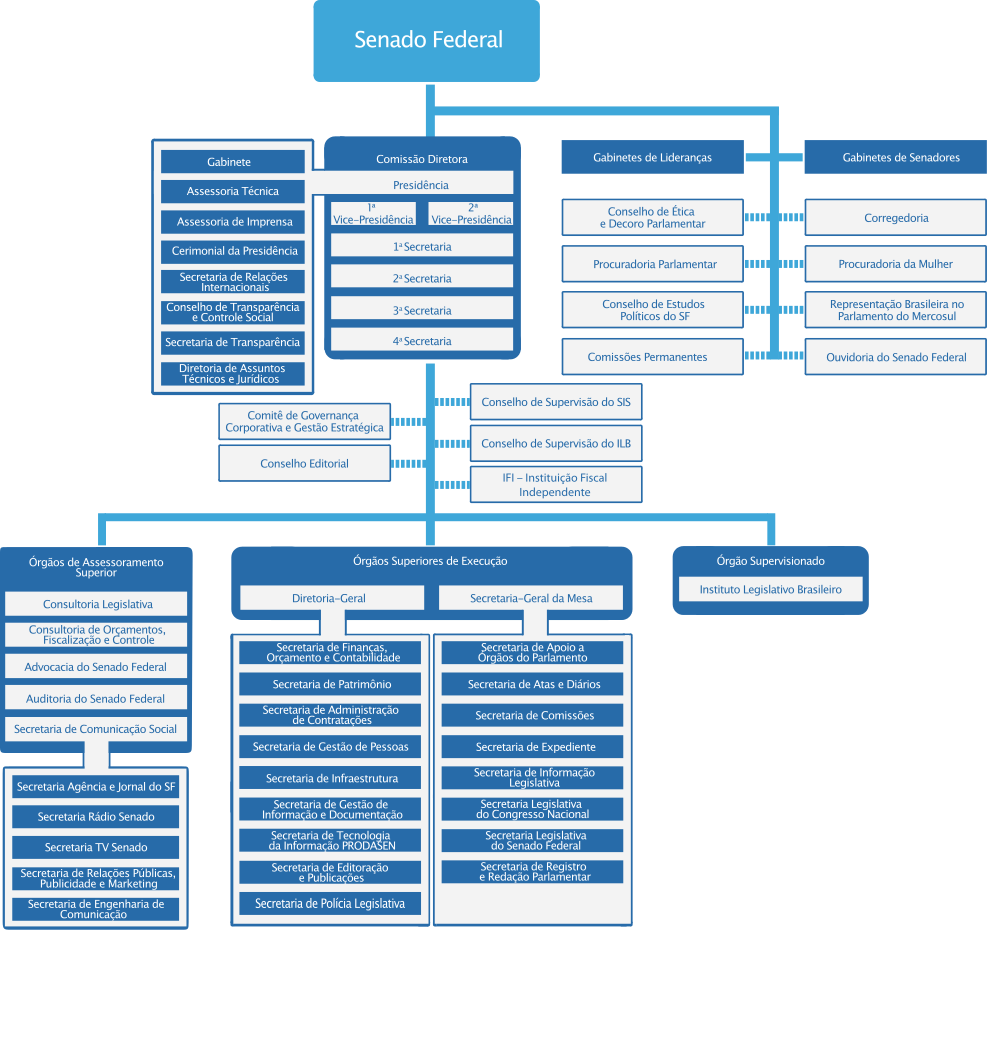
\includegraphics[width=0.8\textwidth]{figuras/organograma_senado.png}
	\caption{Organograma Senado Federal. Fonte: \cite{organograma_senado}.}
	\label{img:organograma_senado}
\end{figure}

\subsection{NMIL}

A Comissão Diretora é composta pelo Presidente, dois Vice-Presidentes e quatro
Secretários. A composição muda a cada dois anos, correspondentes a uma legislatura. É de responsabilidade da Comissão a direção da casa, designando atividades às unidades que dão suporte.

Essas unidades são: Secretaria Geral da Mesa (SGM), representante da atividade fim da casa; e Diretoria Geral (DGER), que, representa as atividades meio da casa. As duas contam com secretarias, às quais delegam atividades exigidas pelo Presidente.

Quando o Presidente da Comissão Diretora necessita de apoio tecnológico, delega esta
atividade à SGM, que, ao receber o problema, começa a definir diretrizes estratégicas para a solução do problema. Após o término da definição das diretrizes, encaminha-as à Secretaria de Informação Legislativa (Sinfleg).

O diretor da Sinfleg atua como Gerente do Projeto, e conta com o apoio da equipe do
NMIL na administração do projeto.

A equipe do NMIL realiza reuniões com as áreas afetadas pelo projeto até conseguir
definir todos os requisitos para o produto que será gerado, após a definição, convoca uma reunião com o Gerente para entrega dos requisitos definidos. O Gerente analisa esses requisitos para saber se são viáveis. Caso não sejam, pede ao NMIL novos requisitos e, só após receber requisitos viáveis, aprova a proposta de solução.

O próximo passo é dado pelo NMIL, convocando reunião com a Secretaria de Tecnologia da Informação (Prodasen). Nesta reunião discute-se os requisitos aprovados e prepara-se o Termo de Abertura do Projeto (TAP). O TAP, deve ser encaminhado pelo NMIL ao Gerente para que este aprove o documento; caso não aprove, pede-se um novo, até que seja aprovado.

Após o Gerente aprovar o projeto, ele o apresenta ao Secretário Geral da Mesa, que é o representante da SGM, para uma aprovação final. O Secretário Geral da Mesa também pode pedir um novo projeto, mas se não for o caso, apenas o autoriza.

Dada a aprovação do Secretário Geral da Mesa, a equipe do Prodasen, responsável pela
construção do produto, dá início à construção do produto, fazendo as entregas de ambiente de homologação (definidas no TAP) ao NMIL, a fim de que este realize testes. Se forem encontrados erros, estes são listados e repassados ao Prodasen para que sejam reparados. Quando não há mais erros, o NMIL dá sua aprovação do produto. Em seguida o Prodasen termina sua parte do projeto e entrega o produto finalizado ao NMIL. O NMIL encaminha o produto ao
Gerente que autoriza o produto e apresenta-o ao Secretário Geral da Mesa.

O Secretário Geral da Mesa, após receber o produto, pode solicitar alterações ao NMIL,
que em seguida encaminha esta solicitação ao Prodasen. A equipe do Prodasen responsável pelo produto faz as alterações necessárias o encaminha de volta ao NMIL, passando pelo processo de teste e aprovação novamente até que o Secretário Geral da Mesa autorize a implantação.

Quando o Secretário Geral da Mesa autorizar a implantação, cabe ao NMIL apresentar
aos usuários o novo Sistema ou as atualizações em sistemas já existentes.

As figuras relacionadas ao mapeamento do processo que ocorre atualmente no NMIL, pode ser vistos no apêndice \ref{ch:figuras}, sendo as figura \ref{img:modelagemProcessoGeral1Parte1} e \ref{img:modelagemProcessoGeral1Parte2} como o processo de pedido da comissão diretora para um novo sistema passando pela SGM, Sinfleg, NMIL e por fim ao Prodasen. As figuras \ref{img:modelagemProcessoGeral2Parte1} e \ref{img:modelagemProcessoGeral2Parte2} se referem ao processo que o NMIL passa até conseguir atingir um sistema estável e que atenda ao pedida da comissão diretora.